\documentclass[tikz]{standalone}
\usepackage{tikz}
\usepackage[compat=1.0.0]{tikz-feynman}
\begin{document}
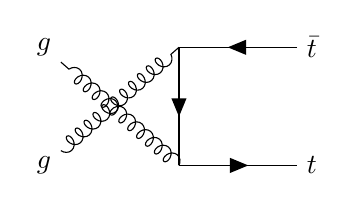
\begin{tikzpicture}
  \begin{feynman}
    \vertex (a);
    \vertex [below = of a] (b);
    \vertex [right=of b] (f1) {\(t\)};
    \vertex [right=of a] (f2) {\(\bar{t}\)};
    \vertex [left=of a] (i2) {\(g\)};
    \vertex [left=of b] (i1) {\(g\)};
    \diagram* {
        (i1) -- [gluon] (a),
         (b) -- [gluon] (i2),
        (f2)-- [fermion ](a) -- [fermion] (b) -- [fermion ](f1),
    };
  \end{feynman}
\end{tikzpicture}

\end{document}